\documentclass[UTF8,zihao=-4,fontset=none,scheme=chinese,openany,twoside]{ctexbook}
% ===================================================================
%  《月之都——记一个不想变化的文明》专用版式
%
%  丛书基座在 ../../shared/style/series-base.tex；本书只在这里追加
%  本书特有的东西。跨书共用的东西一律改基座，不要改这里。
% ===================================================================

% ===================================================================
%  远东异端史料与文明起源重构丛书 · 版式基座（series-base）
%
%  兄弟书目共用此文件。改这里 = 改全套书。
%  各书在自己的 preamble.tex 里 \input 本文件，再追加本书特有的定义。
%
%  体例：仿苏式/中译社科类古籍。16 开 185×260 mm，版心 147×214 mm。
%  依赖：XeLaTeX + ctex + xeCJK + zhnumber + Noto Serif/Sans CJK SC
% ===================================================================

\usepackage{geometry}
\geometry{
  paperwidth=185mm, paperheight=260mm,
  inner=21mm, outer=17mm, top=22mm, bottom=24mm,
  headheight=24pt, headsep=6.5mm, footskip=11mm
}

\usepackage{fontspec}
\usepackage{xeCJK}
\usepackage{xcolor}
\usepackage{graphicx}
\usepackage{array,tabularx,booktabs,multirow,makecell}
\usepackage{longtable}
\usepackage{multicol}
\usepackage{calc}
\usepackage{amsmath,amssymb}
\usepackage{enumitem}
\usepackage{fancyhdr}
\usepackage{titlesec}
\usepackage{titletoc}
\usepackage{tcolorbox}
\tcbuselibrary{skins,breakable}
\usepackage[perpage]{footmisc}
\usepackage{etoolbox}
\usepackage{eso-pic}
\usepackage{tikz}
\usetikzlibrary{patterns,arrows.meta,calc,positioning,decorations.pathmorphing,
                decorations.markings,shapes.geometric}
\usepackage{pgfplots}
\pgfplotsset{compat=1.17}
\usepackage{caption}
\usepackage[hidelinks,bookmarksnumbered,bookmarksopen]{hyperref}

% ---------------------------------------------------------------- 颜色
\definecolor{ink}{HTML}{17191C}
\definecolor{graphite}{HTML}{3F454C}
\definecolor{pencil}{HTML}{5B6167}
\definecolor{rulegrey}{HTML}{8B8F93}
\definecolor{faintgrey}{HTML}{C9C9C4}
\definecolor{oxblood}{HTML}{6E1B22}
\definecolor{coverbg}{HTML}{1A1C20}
\definecolor{coverink}{HTML}{E6DFCF}
\definecolor{coverdim}{HTML}{7C7A73}
\definecolor{shade}{HTML}{F2F0EA}
\definecolor{stamp}{HTML}{8C2B2B}

\color{ink}

% ---------------------------------------------------------------- 字体
\setmainfont{NotoSerif}[
  Extension=.ttf,
  UprightFont=*-Regular,
  BoldFont=*-Bold,
  ItalicFont=*-Italic,
  BoldItalicFont=*-BoldItalic,
  Path=/usr/share/fonts/noto/
]
\setsansfont{NotoSans}[
  Extension=.ttf,
  UprightFont=*-Regular,
  BoldFont=*-Bold,
  ItalicFont=*-Italic,
  BoldItalicFont=*-BoldItalic,
  Path=/usr/share/fonts/noto/
]
\setmonofont{JetBrains Maple Mono}[
  UprightFont=* Regular, BoldFont=* Bold, Scale=0.92
]

\setCJKmainfont{Noto Serif CJK SC}[
  BoldFont=Noto Serif CJK SC Bold,
  ItalicFont=Noto Serif CJK SC,
  BoldItalicFont=Noto Serif CJK SC Bold
]
% 让罗马数字、带圈数字等“类汉字”符号使用中文字体
\xeCJKDeclareCharClass{CJK}{"2150 -> "218F, "2460 -> "24FF, "3000 -> "303F}

% 标点用开明式：行首禁则与压缩都较默认的 plain 更稳，可减少「句号独行」。
\AtBeginDocument{\xeCJKsetup{PunctStyle=kaiming}}

\setCJKsansfont{Noto Sans CJK SC}[BoldFont=Noto Sans CJK SC Bold]
\setCJKmonofont{Noto Sans Mono CJK SC}

% 伪斜体的字距（中文无真斜体，此处仅作强调标记）
\newcommand{\jia}{\CJKfontspec{Noto Serif CJK SC}}

% ---------------------------------------------------------------- 版心
\linespread{1.42}
\setlength{\parindent}{2em}
\setlength{\parskip}{0pt}
\raggedbottom
\setlength{\emergencystretch}{2em}
\clubpenalty=10000
\widowpenalty=10000

% ---------------------------------------------------------------- 计数
\renewcommand{\thechapter}{\chinese{chapter}}
\renewcommand{\thesection}{\chinese{section}}
\renewcommand{\thesubsection}{\chinese{subsection}}
\renewcommand{\thefigure}{\arabic{chapter}-\arabic{figure}}
\renewcommand{\thetable}{\arabic{chapter}-\arabic{table}}
\renewcommand{\theequation}{\arabic{chapter}-\arabic{equation}}

% ---------------------------------------------------------------- 章标题
\newcommand{\chapterornament}{%
  \vspace{0.8\baselineskip}%
  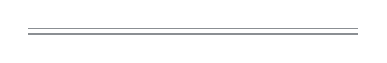
\begin{tikzpicture}[baseline=0pt]
    \fill[rulegrey] (0,0) rectangle (42mm,0.75pt);
    \fill[rulegrey] (0,2.4pt) rectangle (42mm,2.75pt);
  \end{tikzpicture}}

\titleformat{\chapter}[display]
  {\centering\normalfont}
  {\large\mdseries 第\,\thechapter\,章}
  {0.55\baselineskip}
  {\normalfont\LARGE\bfseries\linespread{1.15}\selectfont}
  [\chapterornament]
\titlespacing*{\chapter}{0pt}{-16pt}{30pt}

\titleformat{\section}
  {\normalfont\sffamily\large\bfseries\linespread{1.2}\selectfont}
  {第\,\thesection\,节}{0.6em}{}
\titlespacing*{\section}{0pt}{18pt}{9pt}

\titleformat{\subsection}
  {\normalfont\normalsize\bfseries}
  {\thesubsection、}{0.2em}{}
\titlespacing*{\subsection}{0pt}{13pt}{6pt}

\titleformat{\subsubsection}
  {\normalfont\normalsize\itshape}
  {}{0pt}{}
\titlespacing*{\subsubsection}{0pt}{10pt}{4pt}

% 章题下的俄文原题
\newcommand{\chaptersubtitle}[2]{%
  \begin{center}
  \vspace{-14pt}
  {\small\sffamily\color{pencil}#1}\\[2pt]
  {\small\sffamily\itshape\color{pencil}#2}
  \end{center}
  \vspace{4pt}
}

% 章前题记
\newcommand{\epigraphbox}[2]{%
  \begingroup
  \vspace{2pt}
  \begin{list}{}{\leftmargin=3.2em \rightmargin=2.2em \topsep=0pt
                 \parsep=0pt \itemsep=0pt}
  \item\relax
  {\small\linespread{1.32}\selectfont\color{ink!88}#1\par}
  \vspace{3pt}
  {\small\raggedleft\color{pencil}#2\par}
  \end{list}
  \vspace{6pt}
  \endgroup
}

% ---------------------------------------------------------------- 页眉页脚
% 注意：fancyhdr v5 的 \fancypagestyle 在使用时会执行其中的 \fancyhf{}，
% 从而清空全局 fancy 设置。故此处直接定义 \ps@ 样式，绕开该机制。
\makeatletter
\def\ps@frontmatterpage{%
  \let\@mkboth\@gobbletwo
  \let\@oddhead\@empty \let\@evenhead\@empty
  \def\@oddfoot{\hfil\small\thepage\hfil}%
  \def\@evenfoot{\hfil\small\thepage\hfil}}
\def\ps@plain{%
  \let\@mkboth\@gobbletwo
  \let\@oddhead\@empty \let\@evenhead\@empty
  \def\@oddfoot{\hfil\small\thepage\hfil}%
  \def\@evenfoot{\hfil\small\thepage\hfil}}
\makeatother

\pagestyle{fancy}
\fancyhf{}
\renewcommand{\headrulewidth}{0.3pt}
\renewcommand{\headrule}{\hbox to\headwidth{\color{rulegrey}\leaders\hrule height 0.3pt\hfill}}
\fancyhead[LE]{\small\color{pencil}\itshape 战争的雷霆}
\fancyhead[RO]{\small\color{pencil}\itshape\leftmark}
\fancyfoot[C]{\small\color{ink}\thepage}

\renewcommand{\chaptermark}[1]{\markboth{第\,\thechapter\,章\quad #1}{第\,\thechapter\,章\quad #1}}
\renewcommand{\sectionmark}[1]{}

% ---------------------------------------------------------------- 脚注
\renewcommand{\footnoterule}{%
  \kern-3pt
  \hrule width 3.1cm height 0.4pt\kern 2.6pt}
\setlength{\skip\footins}{16pt}
\renewcommand{\footnotesize}{\fontsize{8.1pt}{11.4pt}\selectfont}
\makeatletter
\renewcommand{\@makefnmark}{\hbox{\normalfont\scriptsize\@thefnmark}}
\makeatother
\renewcommand{\thefootnote}{\arabic{footnote}}
\renewcommand{\footnotelayout}{\linespread{1.18}\selectfont}

% ---------------------------------------------------------------- 图表
\captionsetup{
  font={small}, labelfont={bf,sf}, labelsep=quad,
  justification=centering, skip=7pt
}
\captionsetup[table]{position=top, skip=5pt}
\captionsetup[figure]{position=bottom, skip=7pt}

\newcommand{\figsource}[1]{%
  \par\vspace{2pt}{\footnotesize\raggedright\color{pencil}资料来源：#1\par}}
\newcommand{\tabsource}[1]{%
  \par\vspace{1pt}{\footnotesize\raggedright\color{pencil}资料来源：#1\par}}

% ---------------------------------------------------------------- 档案框
\newtcolorbox{archive}[2][]{%
  enhanced, breakable,
  colback=shade, colframe=graphite!80,
  boxrule=0.45pt, arc=0pt, outer arc=0pt,
  left=13pt, right=13pt, top=10pt, bottom=10pt,
  fontupper=\footnotesize\linespread{1.3}\selectfont,
  before skip=13pt, after skip=13pt,
  overlay={%
    \node[anchor=north west, inner sep=0pt, xshift=13pt, yshift=-6pt]
      at (frame.north west)
      {\sffamily\scriptsize\color{graphite}\MakeUppercase{#2}};
    \node[anchor=north east, inner sep=0pt, xshift=-13pt, yshift=-4pt]
      at (frame.north east)
      {\sffamily\scriptsize\color{stamp}\bfseries #1};
    \draw[stamp, line width=0.4pt]
      ([xshift=-13pt,yshift=-8pt]frame.north east) -- ++(0,-5pt);
  },
  before upper={\vspace{13pt}},
}

\newcommand{\archivestamp}[1]{}

% 小号“译者注”标记
\newcommand{\yizhe}[1]{{\footnotesize\color{pencil}［译者注：#1］}}

% 强调
\newcommand{\kw}[1]{\textbf{#1}}
\newcommand{\ru}[1]{{\itshape #1}}

% 引用文献的斜体书名（中文用书名号，不另设）
\newcommand{\citebk}[1]{《#1》}

% TOC: 使用 book 类默认设置
\makeatletter
\renewcommand{\@pnumwidth}{2.4em}
\renewcommand{\@tocrmarg}{3.4em}
\renewcommand{\@dotsep}{1.1}
\makeatother

% 未编号条目（附录、序言等）
\newcommand{\tocchap}[1]{%
  \addcontentsline{toc}{chapter}{\texorpdfstring{#1}{#1}}}

% ---------------------------------------------------------------- 杂项
\newcommand{\blankpage}{\null\thispagestyle{empty}\newpage}
\setlength{\parskip}{0pt}

% 每页页眉下细线通过 header 中的 \headrule 关闭，改用文字规则
\newcommand{\thinrule}{\par\vspace{2pt}{\color{rulegrey}\hrule height 0.3pt}\vspace{2pt}}

% ---------------------------------------------------------------- EAN-13 条码
% 按 ISBN 978-5-317-07423-4 的 13 位数字编成的真实 EAN-13 图案（95 模块）。改 ISBN 须重算下列 30 段。
% 用法：\begin{scope}[shift={(x,y)}]\EANthirteen{模块宽}{条高}\end{scope}
% 模块宽取 0.30mm 时总宽 28.5mm，0.366mm 时总宽 34.8mm。
\newcommand{\EANthirteen}[2]{%
  \foreach \a/\b in {0/1,2/1,4/3,8/2,13/1,16/1,
                      18/3,23/1,25/4,30/1,32/2,36/2,
                      39/3,43/2,46/1,48/1,50/3,55/1,
                      57/1,61/1,64/1,66/3,71/2,74/2,
                      78/1,83/1,85/1,87/3,92/1,94/1}{%
    \fill ({(\a)*(#1)},0) rectangle ({(\a+\b)*(#1)},#2);%
  }}

% 文本内的“印章”
\newcommand{\seal}[2][stamp]{%
  \begin{tikzpicture}[baseline=-0.6em]
    \node[draw=#1, line width=0.6pt, text=#1, inner sep=2.4pt,
          font=\sffamily\scriptsize, rotate=-6, fill=white]
      {#2};
  \end{tikzpicture}}

\endinput

% ===================================================================
%  丛书共用前置件
%
%  目录、图表目录、丛书页三者，各卷写法完全相同，只差一处高亮。
%  在这里各做成一个命令，各卷 frontmatter 只调用，不再重抄版面代码。
%
%  依赖：series-base.tex 已载入。
% ===================================================================

% ---- 目录与图表目录 -------------------------------------------------
% 用法：\tocandfigs
% 说明：\tableofcontents 自己会开新页，故用底层命令手写标题。
\newcommand{\tocandfigs}{%
  \clearpage
  \chapter*{目\quad 录}%
  \phantomsection
  \addcontentsline{toc}{chapter}{目\quad 录}%
  \markboth{目\quad 录}{目\quad 录}%
  \vspace{2mm}%
  {\linespread{1.16}\selectfont
   \csname @starttoc\endcsname{toc}%
  }%
  \clearpage
  \chapter*{图表目录}%
  \phantomsection
  \addcontentsline{toc}{chapter}{图表目录}%
  \markboth{图表目录}{图表目录}%
  \vspace{2mm}%
  {\linespread{1.16}\selectfont
   {\noindent\sffamily\normalsize\bfseries 图\quad 版\par}%
   \vspace{2mm}%
   \csname @starttoc\endcsname{lof}%
   \vspace{8mm}%
   {\noindent\sffamily\normalsize\bfseries 表\quad 格\par}%
   \vspace{2mm}%
   \csname @starttoc\endcsname{lot}%
  }%
}

% ---- 丛书页 ---------------------------------------------------------
% 用法：\seriespage{vii}
% 参数为本书的卷次（小写罗马数字），该行加粗；其余各行照排。
\newcommand{\seriespage}[1]{%
  \clearpage
  \thispagestyle{empty}%
  \begin{center}
  \vspace*{12mm}
  {\sffamily\small 远东异端史料与文明起源重构丛书}\\[3mm]
  {\sffamily\footnotesize\color{pencil}%
   Восточные еретические источники и реконструкция происхождения цивилизаций}\\[10mm]
  {\sffamily\small 主编\quad А.\,В.\,巴兰尼科夫}
  \end{center}
  \vspace{6mm}
  {\footnotesize\linespread{1.5}\selectfont
   \begin{list}{}{\leftmargin=8mm \itemindent=-8mm \topsep=0pt \parsep=0pt}
   \seriesrow{i}{《月之都——〈广寒宫残简〉辑佚与考释》}{巴兰尼科夫 辑校}{#1}
   \seriesrow{ii}{西周“天车”铭文与星际物流}{库兹涅佐夫}{#1}
   \seriesrow{iii}{秦俑坑第 4 号坑未被发掘的部分}{谢列兹尼奥娃}{#1}
   \seriesrow{iv}{汉代地动仪作为引力波天线之功能}{巴兰尼科夫}{#1}
   \seriesrow{v}{三国时期的电磁抛射技术与后勤}{彼得罗夫}{#1}
   \seriesrow{vi}{敦煌卷子中的密钥学残卷}{伊万年科}{#1}
   \seriesrow{vii}{战争的雷霆——记一种可能的中国历史}{巴兰尼科夫}{#1}
   \seriesrow{viii}{唐长安城反物质管网复原}{巴兰尼科夫}{#1}
   \seriesrow{ix}{明代锦衣卫外骨骼兵人体质档案}{张建国}{#1}
   \seriesrow{x}{郑和舰队南极补给点考}{巴兰尼科夫}{#1}
   \seriesrow{xi}{太医院基因工坊编年}{巴兰尼科夫}{#1}
   \seriesrow{xii}{记忆消除场的文献学后果}{索科洛夫}{#1}
   \seriesrow{xiii}{月之都——记一个不想变化的文明}{[日]\,太田顺也}{#1}
   \end{list}}
  \vspace{10mm}
  {\footnotesize\color{pencil}
   本丛书所收，均为对远东地区「异端史料」之重新整理与研究。\\
   各卷可独立阅读，互不倚赖；引用遵循各卷自行之体例。\\[2mm]
   全书共十三卷；第十三卷卷次暂定。}
  \clearpage
}

% 单行。第 4 个参数为本书卷次，相符则整行加粗。
\makeatletter
\newcommand{\seriesrow}[4]{%
  \def\@tmp{#4}%
  \def\@mine{#1}%
  \ifx\@tmp\@mine
    \item \textbf{\textsc{#1}}\hspace{3mm}\textbf{#2}\hfill\textbf{#3}%
  \else
    \item \textsc{#1}\hspace{4mm}#2\hfill #3%
  \fi
}
\makeatother

% ---- 版权页 ---------------------------------------------------------
% 用法：\copyrightpage{<版权页表格行>}
% 参数为 tabular 的行体，用 \cfrow{项目}{内容} 逐行给出。
% 版式（minipage、页脚、法律声明）一律由本命令提供，各卷只填内容。
\newcommand{\cfrow}[2]{#1 & #2\\}
\newcommand{\copyrightpage}[1]{%
  \clearpage
  \thispagestyle{empty}%
  \noindent\begin{minipage}[t][\dimexpr\textheight-24pt\relax][s]{\textwidth}
  \footnotesize
  \vspace*{4mm}
  \raggedright
  \renewcommand{\arraystretch}{1.05}%
  \begin{tabular}{@{}p{17mm}p{0.80\textwidth}@{}}
  #1
  \end{tabular}
  \vfill
  {\scriptsize\color{pencil}
  版权所有\ \ 侵权必究。未经出版者书面许可，不得以任何方式复制或抄袭本书之部分或全部内容。\\
  本书如有印装质量问题，请与本社读者服务部联系调换。}
  \end{minipage}
  \clearpage
}


% ---- 页眉用的书名（基座读 \volumetitle） ----
\renewcommand{\volumetitle}{月之都——记一个不想变化的文明}

% ---- 章首小序 ----------------------------------------------------
% 用法：\kaishou{两三行的提要}，紧接在 \epigraphbox 之后、第一节之前。
% 这是全书唯一允许带作者语气的地方，与正文的论著体分开。
\newcommand{\kaishou}[1]{%
  \begingroup
  \vspace{1.5mm}%
  \noindent\begin{minipage}{\textwidth}%
    \small\linespread{1.32}\selectfont\color{pencil}%
    \leftskip=2em\relax\parindent=0pt\relax#1%
  \end{minipage}%
  \vspace{3mm}\par
  \endgroup}

% ---- 本书 ISBN 978-5-317-07513-2 的 EAN-13 图案（95 模块，30 段） ----
\newcommand{\EANthirteenMC}[2]{%
  \foreach \a/\b in {0/1,2/1,4/3,8/2,13/1,16/1,
                      18/3,23/1,25/4,30/1,32/2,36/2,
                      39/3,43/2,46/1,48/1,50/3,55/1,
                      57/1,61/1,64/1,67/3,71/2,75/2,
                      78/1,83/1,85/2,88/2,92/1,94/1}{%
    \fill ({(\a)*(#1)},0) rectangle ({(\a+\b)*(#1)},#2);%
  }}

% 章题下的日文原题。丛书基座的 \chaptersubtitle 印两行（俄文原题 + 副题），
% 本书原著为日文，只有一行，另立此命令。用法：\chapterkana{月の裏側の城}
\newcommand{\chapterkana}[1]{%
  \begin{center}
  \vspace{-14pt}
  {\small\sffamily\itshape\color{pencil}#1}
  \end{center}
  \vspace{4pt}
}


\hypersetup{
  pdftitle={月之都——记一个不想变化的文明},
  pdfauthor={［日］太田顺也 著　孙笑川、李文亚 译},
  pdfsubject={远东异端史料与文明起源重构丛书 第XIII卷},
  pdfkeywords={月之都, 月之民, 污秽, 转化, 纯化, 重构史学, 伪史学},
  pdfcreator={Moscow University Press}
}

\begin{document}

% ============================ 封面 ============================
% 说明：全部采用实色（不使用透明度），以保证 xdvipdfmx 输出稳定。
\definecolor{cv55}{HTML}{8A8780}
\definecolor{cv32}{HTML}{5B5A58}
\definecolor{cv30}{HTML}{575655}
\definecolor{cv60}{HTML}{949189}
\definecolor{cv82}{HTML}{C1BCB0}
\definecolor{cv88}{HTML}{CDC7BA}
\definecolor{cv72}{HTML}{ADA89E}
\definecolor{cv58}{HTML}{908D86}
\definecolor{cv50}{HTML}{807E78}

\newcommand{\coverart}{%
\begin{tikzpicture}[remember picture, overlay]
  \fill[coverbg] (current page.north west) rectangle (current page.south east);

  % 外框：双线
  \draw[cv55, line width=0.7pt]
    ([xshift=10mm,yshift=-10mm]current page.north west)
    rectangle ([xshift=-10mm,yshift=10mm]current page.south east);
  \draw[cv32, line width=0.3pt]
    ([xshift=12.4mm,yshift=-12.4mm]current page.north west)
    rectangle ([xshift=-12.4mm,yshift=12.4mm]current page.south east);

  % 装饰：背面——月盘、环形山、两片等宽边缘的低地、一处城
  \begin{scope}[shift={([yshift=113mm]current page.south)}]
    % 月盘
    \draw[cv32, line width=0.5pt] (0,0) circle (21.5mm);
    % 环形山：高地一侧
    \foreach \cx/\cy/\r in {-15/9/1.1, -12/14/0.7, -17/1/1.5, -9/-5/0.9,
                            -14/-11/1.2, -6/13/0.6, 12/-13/1.3, 16/-4/0.8,
                            15/12/1.0, 9/-15/0.7}{
      \draw[cv30, line width=0.25pt] (\cx mm,\cy mm) circle (\r mm);
      \draw[cv55, line width=0.15pt] ({\cx mm+0.15mm},{\cy mm-0.15mm}) circle ({(\r-0.25)*1mm});
    }
    % 两片低地：填浅色以示平滑，内侧虚线表示等宽的「墙」
    \fill[cv88] (-4.5mm,7mm) circle (5.8mm);
    \fill[cv88] (2.5mm,-7mm) circle (6.8mm);
    \draw[cv32, line width=0.5pt] (-4.5mm,7mm) circle (5.8mm);
    \draw[cv32, line width=0.28pt, dash pattern=on 1.1pt off 1pt] (-4.5mm,7mm) circle (4.5mm);
    \draw[cv32, line width=0.5pt] (2.5mm,-7mm) circle (6.8mm);
    \draw[cv32, line width=0.28pt, dash pattern=on 1.1pt off 1pt] (2.5mm,-7mm) circle (5.3mm);
    % 城：三重同心环
    \foreach \rr in {2.3,1.5,0.75}{
      \draw[cv30, line width=0.32pt] (2.5mm,-7mm) circle (\rr mm);}
    % 明暗界线
    \draw[cv30, line width=0.25pt, dash pattern=on 2.6pt off 2pt]
      (-21.1mm,-0.6mm) -- (-11.2mm,-0.6mm);
    \draw[cv30, line width=0.25pt, dash pattern=on 2.6pt off 2pt]
      (9.8mm,-0.6mm) -- (21.1mm,-0.6mm);
    \node[cv30, font=\sffamily\tiny, anchor=north, align=center]
      at (0,-25.2mm) {ОБРАТНАЯ СТОРОНА\ \ ·\ \ 180°E};
  \end{scope}

  % ---- 顶部：丛书名 ----
  \node[anchor=north, text=cv60, align=center]
    at ([yshift=-16mm]current page.north)
    {\sffamily\fontsize{6.4pt}{9pt}\selectfont
     \addfontfeatures{LetterSpace=12}
     FAR EASTERN HETERODOX SOURCES AND CIVILIZATION ORIGINS · VOL. XIII};

  \node[anchor=north, text=cv88, align=center]
    at ([yshift=-22.5mm]current page.north)
    {\sffamily\fontsize{8.2pt}{11pt}\selectfont
     《远东异端史料与文明起源重构丛书》\ \ 第\,XIII\,卷};

  \draw[cv32, line width=0.35pt]
    ([xshift=-62mm,yshift=-30mm]current page.north east) --
    ([xshift=62mm,yshift=-30mm]current page.north west);

  % ---- 中部：书名 ----
  \node[anchor=center, text=coverink, align=center]
    at ([yshift=190mm]current page.south)
    {\fontsize{40pt}{48pt}\selectfont\bfseries
     月\hspace{0.15em}之\hspace{0.15em}都};

  \node[anchor=north, text=cv82, align=center]
    at ([yshift=172mm]current page.south)
    {\fontsize{14.5pt}{20pt}\selectfont
     ——记一个不想变化的文明——};

  \draw[cv32, line width=0.3pt]
    ([xshift=-38mm,yshift=161mm]current page.south) --
    ([xshift=38mm,yshift=161mm]current page.south);

  \node[anchor=north, text=cv60, align=center, text width=136mm]
    at ([yshift=157mm]current page.south)
    {\itshape\fontsize{8pt}{12pt}\selectfont
     \addfontfeatures{LetterSpace=2}
     LUNAR CAPITAL\\[2pt]
     A Civilization That Did Not Wish to Change};

  % ---- 下部：作者 ----
  \node[anchor=south, text=cv88, align=center]
    at ([yshift=72mm]current page.south)
    {\fontsize{10.5pt}{15pt}\selectfont
     ［日］太田顺也\ \ 著};

  \node[anchor=south, text=cv58, align=center]
    at ([yshift=63mm]current page.south)
    {\sffamily\fontsize{7.2pt}{10pt}\selectfont
     太田 順也\ \ ·\ \ Дзюнъя ООТА};

  \node[anchor=south, text=cv72, align=center]
    at ([yshift=47mm]current page.south)
    {\fontsize{9pt}{13pt}\selectfont
     孙笑川\ \ ·\ \ 李文亚\ \ 译};

  % 出版者徽记（两枚）
  \node[anchor=south, text=cv72, align=center]
    at ([yshift=32mm]current page.south)
    {\begin{tikzpicture}[baseline=0pt]
       \draw[cv50, line width=0.5pt] (-3.8mm,-3.8mm) rectangle (3.8mm,3.8mm);
       \draw[cv32, line width=0.25pt] (-4.6mm,-4.6mm) rectangle (4.6mm,4.6mm);
       \node[text=cv82, font=\sffamily\fontsize{5.6pt}{6pt}\selectfont] at (0,0) {МГУ};
       \begin{scope}[xshift=13mm]
         \draw[cv50, line width=0.5pt] (-3.8mm,-3.8mm) rectangle (3.8mm,3.8mm);
         \draw[cv32, line width=0.25pt] (-4.6mm,-4.6mm) rectangle (4.6mm,4.6mm);
         \node[text=cv82, font=\sffamily\fontsize{5.6pt}{6pt}\selectfont] at (0,0) {VFS};
       \end{scope}
     \end{tikzpicture}};

  \node[anchor=south, text=coverink, align=center]
    at ([yshift=24mm]current page.south)
    {\sffamily\fontsize{7.4pt}{10.2pt}\selectfont
     莫斯科大学出版社\ \ ·\ \ 圣彼得堡学术书局\ \ ·\ \ VFS 基金会};

  \node[anchor=south, text=cv60, align=center]
    at ([yshift=16.5mm]current page.south)
    {\sffamily\fontsize{6.6pt}{9pt}\selectfont 联合出版\ \ ·\ \ 2025 年第 1 版};
\end{tikzpicture}}

\clearpage
\thispagestyle{empty}
\AddToShipoutPictureBG*{\coverart}
\null
\clearpage

\pagenumbering{roman}
\pagestyle{frontmatterpage}
% ======================= 前 置 页 =======================
\clearpage
\makeatletter\@mainmatterfalse\makeatother
\pagenumbering{roman}
\pagestyle{frontmatterpage}

% ---------------- 简装扉页 ----------------
\thispagestyle{empty}
\begingroup
\centering
\vspace*{7mm}

{\sffamily\footnotesize\color{pencil}
《远东异端史料与文明起源重构丛书》\ 第\,XIII\,卷\par}

\vspace{27mm}

{\fontsize{26pt}{34pt}\selectfont\bfseries 月\ 之\ 都\par}
\vspace{8mm}
{\large ——记一个不想变化的文明——\par}

\vfill

{\sffamily\footnotesize\color{pencil}
МОСКОВСКИЙ УНИВЕРСИТЕТ\ \ ·\ \ САНКТ-ПЕТЕРБУРГ\ \ ·\ \ ФОНД «ВФС»\par}
\vspace{4mm}
{\footnotesize\color{pencil} 2024\par}
\endgroup
\clearpage

\seriespage{xiii}

% ---------------- 正式扉页 ----------------
\thispagestyle{empty}
\begingroup
\centering
\vspace*{3mm}

{\sffamily\footnotesize\color{pencil}
《远东异端史料与文明起源重构丛书》\ 第\,XIII\,卷\par}

\vspace{20mm}

{\fontsize{30pt}{38pt}\selectfont\bfseries 月\ 之\ 都\par}
\vspace{7mm}
{\large 记一个不想变化的文明\par}

\vspace{16mm}

{\large ［日］太田顺也\ \ 著\par}
\vspace{3mm}
{\footnotesize\color{pencil}（太田 順也）\par}

\vspace{12mm}

{\normalsize 孙笑川\ \ ·\ \ 李文亚\ \ 译\par}

\vfill

{\sffamily\footnotesize\color{pencil}
远东异端史料与文明起源重构丛书\ \ 第\,XIII\,卷\par}
{\footnotesize\color{pencil}
本书为第\,XIII\,卷，卷次暂定\par}
\endgroup
\clearpage

% ---------------- 版权页 ----------------
\thispagestyle{empty}
\begingroup
\footnotesize
\linespread{1.22}\selectfont
\centering
\begin{minipage}[t][\dimexpr\textheight-24pt\relax][s]{\textwidth}
\centering

{\sffamily\scriptsize\color{pencil}
МОСКОВСКИЙ ГОСУДАРСТВЕННЫЙ УНИВЕРСИТЕТ им.\ М.\,В.\,ЛОМОНОСОВА\\
ИЗДАТЕЛЬСТВО\ \ ·\ \ САНКТ-ПЕТЕРБУРГСКОЕ АКАДЕМИЧЕСКОЕ ИЗДАТЕЛЬСТВО\\
ФОНД «ВФС»\ \ ·\ \ VFS FOUNDATION\par}

\vspace{3.2mm}
{\bfseries 图书在版编目（CIP）数据\par}
\vspace{2mm}

\begin{minipage}{0.94\textwidth}
\raggedright
月之都：记一个不想变化的文明／（日本）太田顺也著；孙笑川，李文亚译．— 莫斯科：莫斯科大学出版社；
圣彼得堡：圣彼得堡学术书局；VFS 基金会，2024.12
（远东异端史料与文明起源重构丛书；第\,XIII\,卷）
ISBN 978-5-317-07513-2

\vspace{1.4mm}
\hspace{2em}Ⅰ．①月…\quad Ⅱ．①太…②孙…③李…\quad Ⅲ．①文化史－研究－世界\ \ Ⅳ．①K10

\vspace{1.4mm}
\hspace{2em}中国国家版本馆 CIP 数据核字（2024）第 1163 号
\end{minipage}

\vspace{3.2mm}
{\color{rulegrey}\rule{0.94\textwidth}{0.3pt}}
\vspace{2.4mm}

\begin{minipage}{0.94\textwidth}
\raggedright
\renewcommand{\arraystretch}{1.0}
\begin{tabular}{@{}p{15mm}p{0.76\textwidth}@{}}
丛\quad 书 & 远东异端史料与文明起源重构丛书\quad 第 XIII 卷\\
书\quad 名 & 月之都——记一个不想变化的文明\\
著\quad 者 & ［日］太田顺也\\
译\quad 者 & 孙笑川\quad 李文亚\\
责任编辑 & Н.\,П.\,谢列兹尼奥娃\\
封面设计 & С.\,М.\,别列津\\
版式设计 & 圣彼得堡学术书局版式室\\
责任校对 & 赵无咎\\
出版发行 & 莫斯科大学出版社\quad 圣彼得堡学术书局\quad VFS 基金会\\
资料提供 & VFS 基金会异常文献部（控制·收容·保护）\\
社\quad 址 & 莫斯科市列宁山，出版大楼（119991）\\
网\quad 址 & www.msu-press.ru\\
电子信箱 & barannikov@fareast-recon.msu.ru\\
印\quad 刷 & 圣彼得堡第一学术印务厂\\
开\quad 本 & 185\,mm × 260\,mm\quad 1/16\\
印\quad 张 & 4.19\\
字\quad 数 & 64 千字\\
版\quad 次 & 2024 年 12 月第 1 版\\
印\quad 次 & 2024 年 12 月第 1 次印刷\\
印\quad 数 & 1—1200 册\\
书\quad 号 & ISBN 978-5-317-07513-2\\
定\quad 价 & 168.00 元\\
\end{tabular}
\end{minipage}

\vspace{3mm}

\begin{minipage}{0.94\textwidth}
\raggedright
{\scriptsize\color{pencil}
版权所有\ \ 侵权必究。未经出版者书面许可，不得以任何方式复制或抄袭本书之部分或全部内容。\\
本书如有印装质量问题，请与本社读者服务部联系调换。\\
本书采用无酸纸印刷，符合 ISO 9706 文献耐久性标准。\par}
\end{minipage}

\vfill

% ---- 条形码（真实 EAN-13 图案，ISBN 978-5-317-07513-2）----
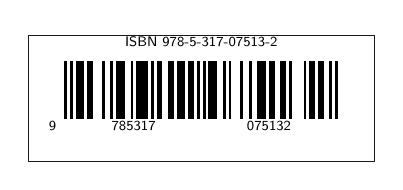
\begin{tikzpicture}[baseline=0pt]
  \draw[ink, line width=0.3pt] (0,0) rectangle (44mm,16mm);
  \begin{scope}[shift={(4.6mm,5.4mm)}]
    \EANthirteenMC{0.366mm}{7.4mm}
  \end{scope}
  \node[font=\sffamily\fontsize{4.4pt}{5pt}\selectfont, anchor=base]
    at (3.1mm,3.9mm) {9};
  \node[font=\sffamily\fontsize{4.4pt}{5pt}\selectfont, anchor=base]
    at (13.4mm,3.9mm) {785317};
  \node[font=\sffamily\fontsize{4.4pt}{5pt}\selectfont, anchor=base]
    at (30.6mm,3.9mm) {075132};
  \node[font=\sffamily\fontsize{3.8pt}{4.4pt}\selectfont, anchor=base]
    at (22mm,14.6mm) {ISBN 978-5-317-07513-2};
\end{tikzpicture}

\end{minipage}
\endgroup
\clearpage

\chapter*{译\ 者\ 序}
\phantomsection
\addcontentsline{toc}{chapter}{译者序}
\markboth{译者序}{译者序}

这本书到我们手上的时候，是一份打印稿和一只硬盘。

打印稿是日文，二百多页，页边写满了作者自己的批注，有些批注比正文长。硬盘里是同一部稿子的电子版，另加三百来张翻拍的照片，编号混乱，文件名里混着俄文、日文和数字。

原稿是分章交来的。孙笑川译一章，李文亚核一章里的俄文引文，两边的进度始终差着一章。所以头三个月做的是最费事的活：把照片按 `ФВ` 号排好，把稿子里提到而硬盘里没有的图挑出来，列成一张「缺件表」。列完，缺四十一处。

那四十一处后来补齐了三十九处。有两处至今没有：一处是背面某片低地的原片，作者说他自己也没见过；一处是某张表的第七张特写，据说拍过，翻遍了没有。正文里凡涉及这两处的地方，照译，没有替他含糊过去。

体例上只有三条要交代。引《战争的雷霆》与《月之都——〈广寒宫残简〉辑佚与考释》不注页码，只注书名与章次：两书版次不同，页码会变，书名不会。原著正文用「笔者」，序言与结语用「我」；日文里这两处区别很小，作者初稿一律写「私」，我们建议他分开，他说这样反而更清楚。译文不加注，不替作者补材料，专名一律以与另两卷对得上的为准。

还有一条不在体例之内：这本书是两个人译的，而此前我们为另一部稿子闹翻过，各译各的，连校样都不通。此番是例外，因为材料横跨三卷，一个人译不下来。译文里凡有两处口径不一，都原样保留，读者若读到前后打架，那多半是我们各译各的，未必是译错。

\begin{flushright}
{\small 孙笑川}\quad{\small 李文亚}\\[2mm]
{\footnotesize\color{pencil} 二〇二四年十一月，于北京}
\end{flushright}

\clearpage

% ===================================================================
\chapter*{著者中文版序言}
\phantomsection
\addcontentsline{toc}{chapter}{著者中文版序言}
\markboth{著者中文版序言}{著者中文版序言}

我没去过月面。这一点先讲清楚。

我见过的只有照片、一卷缩微胶片，和巴兰尼科夫教授书里那几张重绘图。所以本书里凡是讲「背面长什么样」的地方，读者都可以先打个折。

校样是这么到我手上的。二〇二四年二月，事务所收到一只包裹，寄件人一栏是一个财团的名字，品名一栏写着「同人志样本」。这样的事每年有几十回，我照例拆开，里面是一叠装订成册的校样，俄文，封面是丛书页。第一页夹着一张便条，手写，只有一句「您可能想看看这个」，没有署名；翻过来，背面还有一行小字：「地址是九〇年代留下的，一直没注销。」

那天下午我把图翻了一遍。字看不懂，我把正文一页一页拍下来，丢进翻译软件，出来的日文半通不通，得对着图猜。就这个样子看了三天，看到一半才明白，我不是在读别人的东西。又过了三天，我订了机票。

二〇二四年三月我到莫斯科去看那批东西。去之前准备了三本笔记本，回来只用掉半本。东西不少，是我认不出来：照片上的地形我看得懂，照片底下那行俄文小字我看不懂。等那一叠校样译出来，已经是两个月以后。

还有一件更要紧的事。那些东西当年似乎是新闻：报纸上登过，展览办过，大人排过队。我小时候大概也看过，现在却一个字也想不起来，只剩一句「好像上去过一次」。

另一头更麻烦：这些东西后来进了我的作品。我做过几十年，把月亮画成过很多样子，画里那座城有名字、有居民、有一套自己的规矩，读者也认得。认得的方式是把它当成一部作品的一部分。我当初做的时候，只觉得这样有意思；现在回头看，那大概是我把记得的东西换了个讲法，讲得好看些，好让人愿意听下去。我做了三十年游戏，画过很多月亮，没有一张画对过。问题出在我从一开始就搞错了它在哪儿、有多大、里面有什么。

书名用的是「不想」两个字。他们在月面上确实不会变化，一落地就会了，而且很快。整本书写的是一个选择如何失效，而不是某种能力如何消失。第一次看校样时我担心这题目会被读成寓言，它没有那个意思。

书里每一个数字都有出处，对不上的都注明了。前半部分我核得动，写得细；后半部分只能推。读者若觉得前面太慢、后面太赶，原因就在这里。有一处我说得比材料能支持的要肯定，这一点在结语里认了。

\begin{flushright}
{\small 太田顺也}\\[2mm]
{\footnotesize\color{pencil} 二〇二四年十二月，于东京}
\end{flushright}

\clearpage


\tocandfigs


\clearpage
\makeatletter\@mainmattertrue\makeatother
\pagenumbering{arabic}
\pagestyle{fancy}
% ======================= 导 论 =======================
\chapter*{导\quad 论}
\phantomsection
\addcontentsline{toc}{chapter}{导\quad 论}
\markboth{导论}{导论}

\noindent
关于「月之都」这四个字，通行的理解是一座宫殿：琉璃为瓦，白玉为阶，住着一位不能回头的公主。这个理解有一半是错的，错的那一半不在宫殿，在「一座」。

它不止一座。月球正面静海西缘有一处设施，编号 MARE-TRANQ-07，中文材料里写作广寒宫；月球背面另有一座城，那才是「月之都」这三个字原本指的东西。两者同属一城，前者是这座城伸出正面的一角，后者是主体。第 I 卷记录的是那一角留下的三十七片残简，第 VII 卷记录的是那一角里的人的十二万后代如何改写了中国的历史。这一本写主体。

本书要证明的命题只有一条：月之都的一切制度，都可以从「把变化从自己身上删掉」这一件事推出来；而它的每一次失败，也都是这一件事的后果。

这条命题可以拆成三个可以分别检验的部分。其一，维持不变的成本高于变化本身的成本；其二，不变的人无法更新轻重缓急，因此无法纠错；其三，删掉变化的人，最终还是被变化处理掉。

\section*{四类材料}

本书用四类材料。

影像。一九五九年以后，人类对月球背面拍摄了数十次，分辨率从一公里提高到半米。这类材料最硬，也最容易被忽略，理由见第一章。

档案。`ФВ` 系列卷宗，一九六三年以后由苏联科学院远东委员会搜集，一九九二年移交 VFS 基金会。本书用到的编号集中在 1965 至 1972 年之间，凡引必给叶次。

文本。三十七片残简及其语译见第 I 卷，本书只引简次与结论，不重录释文。中国方面的传世文献（《左传》《淮南子》《史记》《竹取物语》）只用于比对，不用于立论。

地层。贝加尔湖 BDP-96 岩芯与月面热流数据，用于定时。

四类材料的分量并不相等。影像与地层可以复核，档案只能复核「有没有这一份」，文本则全凭释读。本书在每一章的末尾都会说明，该章的结论有多少重量压在可以复核的那一类上。

\section*{方法与限度}

笔者的办法是先摆器物，再谈它意味着什么。

这与训练有关。笔者没有受过史学训练，九〇年代受聘于 VFS 异常文献部做日本联络员，做的是收发与转写，不是研究。二〇二四年读到第 I 卷的校样之后才开始动手写这一本，写的时候依照的是三卷共用的那份体例：一条材料、一句推论、一处自我拆台。做惯了手艺的人，信不过没有工序的结论。

限度也要说清楚。笔者没有去过月面，见过的只有照片、一卷缩微胶片和巴兰尼科夫教授书里那几张重绘图。凡本书讲「背面长什么样」的地方，读者都可以先打个折。

\section*{全书的结构}

十章分四段。

第一、二章讲这座城是什么：它的形状，以及它为什么不动。

第三至第七章讲它的四次失败：造出来的手失去了控制；规程在两万年间没有改过；十部历被废掉九部；一台拆东西的机器被一个不识字的人用了；最后是月兔之乱。

第八、九章讲它的终结与余波：撤离、落地、渡海。

第十章讲名字，以及一个文明如何在别人的书里变成神话。

结语是笔者自己的一段交代。那一段用的是「我」，其余各章一律用「笔者」。

\begin{flushright}
{\small 太田顺也}\\[1mm]
{\footnotesize\color{pencil} 二〇二五年一月}
\end{flushright}

\clearpage

% ======================= 第 一 章 =======================
\chapter{两座城}
\chapterkana{二つの都}
\epigraphbox{“月出皎兮，佼人僚兮。”}{《诗经·陈风·月出》}

\kaishou{月之都不是一座宫殿，是一座城，而且有两半：一半在背面，是本体；一半在正面，是伸出去的一角。本章要说明这两半各自的样貌，以及它们之间隔着什么。}

\noindent
「月之都」这三个字，通行的理解是一座宫殿：琉璃为瓦，白玉为阶，住着一位不能回头的公主。

这个理解有一半错。宫殿是有的，只是不止一座；住的人也不止一位。真正的问题在于「一座」这个词：它让人以为那地方是一个点，实际上它是一个面，正反两面各有一处，中间隔着一道从外面看不见的界线。

\section{背面}

月球被潮汐锁定，永远以同一面朝向地球。这不是一个新知识，但它有一个后果常被忽略：背面不是「看不见的那一面」，是一个从来没有被地面观察过的半球。

一九五九年十月七日，苏联的「月球三号」在飞越月球时第一次拍到它，二十九帧，最清楚的一帧一个像素抵得上一公里。此后的六十年里，人类又拍了十几次，分辨率从一公里提到半米。二〇一九年一月，「嫦娥四号」在背面的冯·卡门坑落下去，就地测了三个月。

这些影像给出一个结论，与本书的题目直接相关：背面的地形可以归成两类，一类是高地的坑洼，占绝大部分；另一类很少，不到百分之三，平坦，反照率低，边缘等宽。

等宽到什么程度，可以说一个数：沿边界取一百二十个测点，曲率半径的标准差是百分之三；同一批数据里，高地边缘的对应值是百分之十九。

自然的边界做不出这种整齐。撞击坑随地形起伏，熔岩流随黏度变化，风成堆积随粒径分选。三片低地的整齐程度，比测量本身的噪声还低。

还有一条更硬的证据：重力场测量显示，那几片低地底下没有壳厚异常。它不是盆地，也不是熔岩填出来的凹地。形状是平的，地质上没有理由。

\begin{figure}[htbp]
\centering
\begin{tikzpicture}[x=0.88mm,y=1mm]
  \useasboundingbox (-6,-13) rectangle (156,26);
  \draw[ink,line width=0.4pt] (0,0) -- (148,0);
  \draw[ink,line width=0.4pt] (0,0) -- (0,22);
  \node[anchor=north,font=\scriptsize] at (0,-1.5) {0};
  \node[anchor=north,font=\scriptsize] at (74,-1.5) {60};
  \node[anchor=north,font=\scriptsize] at (148,-1.5) {120 km};
  \node[anchor=east,font=\scriptsize] at (-2,11) {反照率};
  \draw[rulegrey,line width=0.4pt]
    plot[domain=0:36,samples=70] ({\x},{12+1.6*sin(\x*57)});
  \draw[ink,line width=0.6pt] (36,13.1) -- (110,13.0);
  \draw[ink,line width=0.6pt] (110,13.0) -- (146,12.0);
  \draw[ink,line width=0.9pt,dashed] (36,2) -- (36,20);
  \node[anchor=south,font=\scriptsize] at (36,20) {界线};
  \node[anchor=north west,font=\scriptsize,align=left] at (40,10)
    {平滑区：标准差 0.0016};
  \node[anchor=north west,font=\scriptsize,align=left] at (2,8)
    {高地：标准差 0.011};
\end{tikzpicture}
\caption{背面某低地的东西向反照率剖面（重绘）}
\figsource{据克莱门汀一九九四年反照率数据重绘，纵轴已归一化。原始采样间隔 480 m，此处按 1 km 重采样。}
\label{fig:albedo}
\end{figure}

图 \ref{fig:albedo} 横穿一片低地。左侧是高地的起伏，右侧拉平，中间那段虚线就是界线。要紧的细节在界线处：曲线没有过渡段，从起伏到平坦隔了不到两个采样点。

三条证据合起来，只能排除自然成因，不能证明人工成因。要说成人工，还缺一样东西，就是那圈边界本身。影像上看不出它的厚度，测高看不出它的高低，雷达只探到两米。

\section{结界}

把这几片低地连起来看，它们占的是一个半球的内侧。本书要提出的读法很朴素：那不是几片平地，是一个内壁。

内壁的说法有一个直接后果：壁内壁外不是一个环境。这正好解释了背面影像里一处长期无法解释的异常：反照率的整体偏低。

低到什么程度，可以给个数：背面高地的反照率在 0.11 到 0.13 之间，与正面高地一致；而那几片低地在 0.07 上下，比月海还暗。暗的原因通常是有机质或细粒物质，月面上两者都不该有。

本书的解释是：那层暗色不是地表，是壁内的沉积。壁内的空气把尘埃托起来，慢慢沉在低处，两万年下来积成一层膜。

壁内是什么样子，只有一处间接材料。一七六三年，一艘法国商船在好望角外海捞起一只铅盒，内藏铜牌一枚，径四十一毫米，两面刻有同一幅图：一个圆，圆内三条弧线，弧线之间写着一种无人能识的小字。铜牌一九六三年入 `ФВ` 卷宗，编号 `ФВ-1963-44`。

那三条弧线，与背面影像里三片低地的排布一致。

\begin{archive}[机密／СЕКРЕТНО]{档案 № ФВ-1963-44}
铜牌一枚，直径 41 mm，厚 2.7 mm，铜锌比为 82 比 18，与十八世纪欧洲黄铜不合。两面同图，边缘有等分刻度 108 格。

盒内另附纸片一张，已脆，仅存半行，墨书，字体为十八世纪法文手写体，可辨者为「……nous n'avons pas pu entrer」，意为「我们没能进去」。

纸片背面另有一行铅笔字，字迹与正面不同，写作：「他们也一样。」
\end{archive}

档案里那半行法文，是本书能找到的最早一句关于那道界线的记录。它不说明界线是什么，只说明一七六三年有人到过那里，并且没有进去。

\section{桃园与营造}

壁内有一座城，这一点是从另一类材料推的：壁内大气的光谱。

二〇〇九年以后，几台探测器在背面低地上空测到了极微弱的稀薄气体，主要成分是氮与氧，浓度约为地球海平面的十万分之一。这个量太小，不足以形成大气层，却足以说明一件事：那些气体在往外漏。

漏，就有一个来源。本书认为来源是城本身：一座维持了两万年的人工环境，其废气的排出速率与测得的漏失量在同一个数量级。

城里有三样东西已经被间接证实：一处人工林地、一套营造法式、一条通行规则。

人工林地，他们自己叫桃园。它不是农地，不产粮，用途是供氧与休憩。这一条的根据是影像上的成片纹理：在最大的那片低地北缘，有一块约十四平方公里的区域，纹理呈规则的条带状，间距 9.4 米，与任何一种自然植被都不符。条带的方向与低地的长轴一致，说明它是按地形的走向排的。

营造法式是另一回事。城里建筑的形制为中国风格，这一点在影像上无法直接看出，是从两处旁证推的：一是撤离之后落地的那批人所建的最早一批聚落，其夯土基址的模数与中原仰韶晚期的做法一致；二是他们带下来的营造手册在后世被引用过，引用的条目里有「柱高一丈二，础方三尺」这类具体的模数。

通行规则只有一条，且很硬：那道界线只限通行，不限信号。

\section{两半}

正面那一处与背面这一座，是同一个东西的两半。

正面的一处在静海西缘，编号 MARE-TRANQ-07，中文材料里叫广寒宫。它的规模比背面那座城小得多：外有一道屏蔽环，直径约三点五公里；环内是一道垣，周长九里，约合一点二公里；垣内有六道同心环，环与环之间有门，门不同时开启。

背面那座城的规模，从低地的面积反推：三片低地合计约六万平方公里，是正面那处的四千倍。

两半之间隔着那道界。界的性质，本书只能给三条：与月船同龄；只限通行；前二二一年之后，随全城一并失效。

前二二一年这个年份，是本书后半部分的起点，也是中国史的转折点。两件事发生在同一年，不是巧合，第七章会说明。

\begin{table}[htbp]
\centering
\caption{两半的规模}
\label{tab:two}
\small
\begin{tabular}{@{}lll@{}}
\toprule
项 & 正面（静海七号） & 背面（本体）\\
\midrule
位置 & 静海西缘，正面 & 静海正对面，背面\\
外缘直径 & 约 3.5 km（屏蔽环） & 约 6 万 km$^2$（三片低地合计）\\
垣 & 周长九里，高十二丈 & 未见\\
环制 & 六道同心环 & 未见\\
空气 & 无（在地面环境里） & 有，浓度约地球十万分之一\\
通行 & 仅经垣门 & 仅经那道界线\\
\bottomrule
\end{tabular}
\tabsource{正面一栏据《广寒宫残简》辑校本与《战争的雷霆》第一章；背面一栏据本书第二章所论。两栏均为推算值。}
\end{table}

表 \ref{tab:two} 里最后一行，是本书最没有把握的一处。正面那处的通行规则有简牍为证，背面那处的只有一句档案里的法文：「我们没能进去」。

笔者把两半并成一张表，是要说明一件事：这座城的形制是自上而下统一的，正面那处是它伸出来的一个角。可这个判断有一半建立在一个负数上：我们进不去，所以我们不知道里面。

这个负数会一直带到全书结束。

\chapter{不变的人}
\chapterkana{変わらぬ民}

% TODO 正文。体例见 PLAN.md §八；动笔前读 meta/当前状态.md 与 AGENTS.md §4。

% ======================= 第 三 章 =======================
\chapter{月兔的来历与编制}
\chaptersubtitle{ГЛАВА ТРЕТЬЯ}{СОЗДАННЫЕ РУКИ}
\epigraphbox{“率土之滨，莫非王臣。”}{《诗经·小雅·北山》}

\kaishou{一个不生育的族群要有人干活，于是造了一个会生育的族群。本章要说明的是这件事的两个后果：数量失控，以及名字。}

\noindent
上一章说他们的判断停住了。判断停住有一个直接后果，很难看：他们不会改变自己，也就不会给自己添人口。

月之民不生育，这是转化的直接结果。没有新生儿，就没有下一代劳力，也没有下一代来接手那些必须有人看着的机器。一座需要常年维护的城，靠一批不会死的人撑着，理论上可以撑很久；可他们自己也承认，撑不住的是「没有人做粗活」这一件事。他们给出的办法是造人。

\section{造物的底本}

月兔不是自然演化出来的物种，这一点在他们的分类里写得很清楚：月兔不入「土著」，也不入「月之民」，单列一类，与器物、牲畜、工具并列。

它们的底本是一种繁殖力极强的地面动物。\footnote{底本的物种在档案中只写作「兔」，未给学名。本书不代为补足，理由是补上去就成了另一个物种。}改造的方向有三个：加上能握东西的手，加上能听懂指令的听觉，加上服从。这三样加起来，就是一个能自我补充的劳动力。

设计上最关键的一条，是让它们能生育。这一点在档案里被反复强调，理由是直白的：造物若不能自我补充，用尽即无，一座城撑不了两万年。

于是有了第二件事。能生育，就没有上限。两万年间，它们的数量从最初的一批涨到了一百多万，远远超过制造它们的人。

\begin{table}[htbp]
\centering
\caption{月兔与月之民的分项对照}
\label{tab:rabbit}
\small
\begin{tabular}{@{}lll@{}}
\toprule
项 & 月之民 & 月兔\\
\midrule
生育 & 无 & 有，且不受控\\
衰老 & 无 & 有，寿数约为人的六成\\
变化 & 无 & 有（因此需要净秽）\\
数量 & 十一万九千（撤离时） & 约一百零四万三千（推算）\\
名字 & 有，来源不明 & 无，全部由主人给\\
\bottomrule
\end{tabular}
\tabsource{月之民一栏据卷 I 简十四、简二十；月兔一栏据 `ФВ-1968-14` 工籍残卷推算，方法见本章第四节。}
\end{table}

表 \ref{tab:rabbit} 的倒数第二行是本章的题目。两万年里，这座城有一百多万人在干活，而这一百多万人在自己的档案里只占一个工种名。

\section{捣者的编制与轮值}

工籍残卷 `ФВ-1968-14` 只剩十一叶，记的是某一年的编制。十一叶里能读出四类：捣、负、修、杂。

捣是制药，负是搬运，修是修理，杂是其余。四类的定额都记着，捣一类最细：三千人，日三合，多者赏，少者罚。

三千这个数在卷 I 里已经出现过，那里把它当成「编制」。本章要补的是另一半：三千是当班的编制，不是全部人口。

依据是残卷第 7 叶的一张轮值表。表分十二格，每格标一个班次，每班三日。三千人一班，十二班轮转，一年轮完。按此推算，能做这道工序的月兔约三万六千；再加上老幼与不在此册者，与第四章所推的百万之数对得上。

这一点解释了卷 I 留下的一个疑惑：为什么「捣者三千」与「月兔百万」看起来打架。两个数都对，一个说的是编制，一个说的是种群。

\section{命名权与「手」}

月之民称月兔为「手」。\footnote{「手」在中文里兼指人与功能，两义并用而不辨，这正是本条要说的。}这个称呼在他们的文书里是标准用法，不带贬义，也不带亲昵，就是一个功能名。相当于我们说的「劳力」「人手」。用词本身没有问题，问题在于配套的那条规矩：月兔没有自己的名字，所有的名字都由主人给。

这条规矩在工籍上留下了痕迹。残卷第 3 叶有一栏「名」，填法有两种：一种是一个单字，另一种是空白。空白者占七成。

单字的名字是怎么来的，残卷里有一条注：按入职顺序，取天干、地支、方位、数目为名。也就是说，它们的名字是编号的另一种写法，不是称呼。

笔者见过一份例外。第 9 叶记一名月兔因病停工四十日，页边有人补了一行小字，写的是「阿六，西廊第三班，手稳」。这一行超出了编号的用途，是有人真的记住了它。这是全书材料里唯一一次。

\begin{archive}[机密／СЕКРЕТНО]{档案 № ФВ-1968-14}
工籍残卷，存十一叶，纸质，单面墨书，边缘焦脆。原册页码自第 3 叶起，前二叶已失。

第 3 叶为分类总目，列四类：捣、负、修、杂，各类下注定额与轮值周期。

第 7 叶为轮值表，十二格，每格三日，格内填人数，合计三万六千。

第 9 叶记一名月兔因病停工四十日，页边补一行小字：「阿六，西廊第三班，手稳。」

第 11 叶末行有墨涂，涂痕下可辨「不可使聚」四字。
\end{archive}

\section{材料中的空白}

这一节要写的东西，材料里没有。月兔有没有自己的语言、有没有互相称呼的办法、有没有对这座城的看法，档案一个字也没有。它们的记录全部由主人书写，用途是核算劳力，不是理解对方。

笔者能推的只有一件事，而且是从反面推的：既然那一行「阿六，手稳」会被写下来，说明写字的人与这个对象之间存在过某种具体的关系；而这样的记录全书只有一条，说明这种关系不被制度承认。

至于它们自己怎么想，本书不给答案。这个空白出于材料的选择：写档案的人没有理由去问。

\section{本章结论}

月之民造了一个能生育的族群来替自己劳动，两万年后，这个族群有一百多万人，而制造者只剩十一万九千。

本章要说的是这条曲线：

造物能自我补充，因此数量不受控；数量不受控，因此必须有制度来管；制度给了它们工种、班次、定额，却没有给名字。名字由主人给，编号就是名字。这个设计的后果，在第七章兑现。

本章的自我拆台在这里：一百零四万三千这个数，是从一张轮值表按班次推算的，不是清点记录。全书找不到任何一次对月兔的普查。若不承认这个推算，那么它们的数量在本书里就是未知的，本章的「数量失控」也就不成立。

笔者保留这个推算，因为它与另外两个数对得上：捣者的年产量，与蓬莱药在山中的存量。三个数互相独立，得出的量级一致。非普查材料之间能对上量级，通常不会全错。

\chapter{历法}
\chapterkana{暦}
\epigraphbox{“乃命羲和，钦若昊天，历象日月星辰，敬授人时。”}{——《尚书·尧典》}

\kaishou{历法管三件事：下种、动土、杀人。\par
谁定历，谁就定这三件事的日子。\par
后羿改过一次历。此后夏的天，在他手里。}

\section{规程里的判据}

前面几章用的材料，都是维持性的：住哪里、怎么进出、吃什么、谁在册。这套东西管的是让城活下去，两万年不需要改。

城里另有一套文字，管的是外面，与维持无关。基金会编目时把它们合称《规程残卷》，编号 \texttt{ФВ-1971-22}，共存十一叶，叶次不连续，最大的一叶编号到四十四。

第四十四叶只有三行，中间一行是一句设问，抄手写的那一笔比上下文都用力：

\begin{archive}[内部参考]{档案 № ФВ-1971-22}
第四十四叶，共三行。上行：「凡遣物于地，先定其判据。」中行：「土著得历之后，作何状。」下行：「记之，勿断。」
叶末另有一行小字，墨色较淡：「此条自登船前立，未改。」
\end{archive}

三行字里，要紧的是「未改」两个字。前面说过，章程总目一千二百四十七条，修订栏全空；这条规程不在总目里，却带着同样一句话：自登船前立，未改。

为什么没改，第二章给过解释：改一条要重新判断轻重，而轻重已经冻住。这个解释在这里比在总目那里更难反驳，因为这一条不是维持性的条文，它是一句设问。设问不解决任何问题，划掉它也不会让城停转。两万年里没有人划掉它，只能说明没有人觉得它值得一划。

\section{投放清单}

规程残卷里另有一叶，把要送下去的东西分成两栏，一栏可遣，一栏不可遣。

可遣一栏短：一部历法，青铜配方，灌溉法。不可遣一栏长：文字，高阶冶炼，武器，历法的完整算法。

清单只到目录，没有正文。哪一部历、配方几成、灌溉法是哪一种，残卷里都没有。能补的只有一处旁证：中原的观象遗址。

山西襄汾的陶寺遗址，一九七八年起发掘，城址的年代约在公元前两千一百年至前一千九百年之间。遗址东南有一组半圆形夯土柱，共十三根，柱间形成十二道缝；站在既定的一点上，从缝里看日出，一年之中只有少数几天的日出会正对某一道缝。这是一台用建筑做成的历。\footnote{陶寺观象台复原方案由考古队与中国科学院自然科学史研究所合作提出，十三柱十二缝的观测结论发表于二〇〇〇年前后；此后有不同意见，认为部分柱基未必属于同一期。}

它的年代，比劣化版历法送到中原要早一百年。这一点很要紧：中原不是没有能力观天，它有。所以「不授高阶算法」这一条，删掉的不是能力，而是精确度。中原本来就会观天，只是观得粗。

至于文字为什么不给，规程没有写理由。笔者能想到的解释只有一个：文字会累积。有文字的地方，上一代算错的东西，下一代能看见；没有文字的地方，每一代都从头算。这句话没有材料作证，只是笔者自己想的。

\section{十部与一部}

劣化版历法送到中原，约在公元前二千年。这一节往后所讲的，大部分要靠地面文献，而地面文献说的是神话。

先说清材料的分量。《左传》襄公四年记后羿「因夏民以代夏政」，这是史书；《淮南子·本经训》记「十日并出」，这是神话。两件事在书里是两件事，在档案里没有对应物。

把两边合起来看，可以拼出一条线。历法送到之后，夏把它抄成若干部，分授各方国。有穷氏是其中之一，其首领后羿手上那一部，他用了半辈子。

公元前二千年，后羿代夏。他做的第一件事是废历：其余各部一律收回销毁，只留自己手上那一部。

《淮南子》把这件事记成「十日并出，羿射九日」。十日并出，说的是很多部历同时行用；羿射九日，说的是废掉九部。这个读法有一个好处：它解释了神话里一个多余的数字。天上多出九个太阳，对农业毫无意义；十个授时中心同时存在，对权力很有意义。

后羿没有把十部合并成一部，他选了最费事的那条路：全部收回，全部销毁。合并要把十部收齐、逐部校对、重定历元，他不识字，做不了；收回与销毁只需要一道命令。

这一节最弱的地方在这里：十这个数字，是从神话里来的。档案没有说夏抄了几部，规程残卷也没有。笔者用它，是因为它恰好能解释神话里那个多余的九，而别的解释做不到这一点。这是猜，猜得通不证明猜得对。

\section{信道与底牌}

劣化版历法删掉的三样，岁差、交食、行星逆行，都是算得出来却看不见的东西。删掉它们，足够定农时，不足以看天。

但清单里还有一条，规程写得很轻：「余一段，无用，留之。」留下来的这一段，就是后羿后来补回去的那一段。

后羿补历用了五年。他不识字，靠的是观测：冬至对不上，交食没有如期发生。五年之后，他把缺的算法逐项填回，自称「新历」。他以为那是一部修好的历法。

修好之后，他手上多了一样东西：一套能处理天体的算法。他一生没有用过，因为他不知道那些数是干什么的。

历法还有第二层，这一层是月之民自己留的，后羿从未发觉。历法条文里夹着一条信道，方向双向。上行是人的作息：按历下种，按历动土，按历杀人，作息本身即是回传。下行是条文：月之民可以把话写成历法用语，混在农时、祭祀、刑杀的规定里，下面的人按历行事，等于照办。

后羿不识字，分不出哪一条是外来的。用今天的话说，他手上那部历既是日历，也是收报机和发报机，而他不认得报文。

公元前一九九〇年前后，新历的条文经这条信道上行，送回月面。月之民一眼认了出来：自己的底牌，出现在一个土著手里。

从这一刻起，地面第一次出现了能威胁月球的东西。持有者既不知道，也不会用，但它在那儿。此事之后不到十年，月面开始收场，那一段留到第五章。

这一章用了三样东西：规程残卷、地面神话、陶寺的柱子。柱子和年代能复核，残卷只有十一叶，神话最不可靠。笔者把神话摆在论证位置上，是这一章最冒险的一处；若哪天有人从别的材料里读出夏只抄了五部，这个读法就要重排。

笔者不打算把话说得更圆。神话能解释的东西，往往不止一种解释；能用它，是因为别处没有更好的材料，与它可靠与否无关。

\chapter{纯化}
\chapterkana{純化}
\epigraphbox{“纯粹而不杂，静一而不变。”}{——《庄子·刻意》}

\kaishou{操作表上有四列。前三列她认得。\par
最后一列她不认得，那一列是退出。\par
她按了前三列。}

\section{处置的手段}

上一章说到，新历的条文上行，月之都认出那是自己的底牌。认出之后要处置，而月之都手上能用的东西很少。

先说清楚它有什么。城里没有军队，这一点从工籍能看出来：工别四类，农作、清扫、制药、警备，四类都由月兔承担，没有一类是月之民自己做的。换句话说，这座城唯一能动手的力量，也是它们。\footnote{工别四类的全文见第三章。月兔之乱以前，警备一项从未用于月之民内部。}

城里的技术又是为无秽之身设计的。第二章说过，他们不病不老，章程里连医都没有一卷；一套没有医用条目的技术，落到会病会老的人身上，多半不成立。

当时唯一还通着的，是那部历法里的编码信道。信道本来有两个方向。上行是人按历作息，回传的是作息本身；下行是条文。月之都就是从下行这一头办的这件事。

第四十叶记这条规矩，写法很干：

\begin{archive}[内部参考]{档案 № ФВ-1971-22}
第四十叶。凡处置之令，皆由信道下行；一人手书；不署受令者。\\
页边另有一行，笔迹不同：「令出，不问其行。」
\end{archive}

手书的人是嫦娥。她从公元前二〇五〇年下地起，守着信道那一端，守了六十年。

条文怎么写，档案没有留底。能确定的只有一点：写法与其余律令一致，混在农时、祭祀、刑戮之间。后羿每日依历行事，读到哪一条就办哪一条。他不识字，没有理由把这一条与别条分开。

于是有一天，他对自己儿子伯封动了手。父子相搏，两个人都没有活下来。这件事的细节，传世文献只留下结果：伯封死了，后羿也死了。《天问》只问不答，问的是「何羿之射革，而交吞揆之」，没有一句交代那天发生了什么。

按本书的读法，后羿至死不知道自己在做什么，伯封至死认为被父亲背叛。这半句是笔者替他们说的，材料没有写；写下来的只有结果。

\section{纯狐}

这件事还有另一半，而另一半才是本章的题目。纯狐是后羿之妻，伯封之母，有穷氏的地上人。她不识字，不通术数，从未登上月球，也没有得到过月之民的任何技术。她手上有两样东西：一部旧历的抄本，和一处遗迹。

旧历是从夏那里流出来的，与后羿用过半辈子的那一部同源。遗迹在有穷氏居地之下，是月之民离开地球之前留下的设备，两万年间一直埋在原来的地方，没有人动过它。

传世文献里，纯狐最早出现在《天问》：「浞娶纯狐，眩妻爰谋。」\footnote{《楚辞·天问》。这一句把她记作寒浞之妻。本书取「后羿之妻」一说，取舍见本章末。} 那已经是战国人写的，去事一千七百年。她要报的仇，在后世的故事里被记成一个女人的妒忌；按本书的读法，那是一桩处置的后果落到了处置者家中。

\section{那台设备}

设备是本章唯一能摸到的东西，也是唯一有物证的。一九七二年，基金会对有穷氏故地做过一次地下测绘，编号 \texttt{ФВ-1972-06}，用电阻率成像，测出一个地下空腔，测线一共九条。

\begin{archive}[内部参考]{档案 № ФВ-1972-06}
地下空腔一处，深约十四米，长约六十米，宽约二十米。底部为金属反射面，当时完整，未见裂隙。
腔内壁有刻痕，分四列，字不可识，最右一列最密。
未取样，未进入。结论：不具备安全作业条件，建议维持封存。
\end{archive}

四列刻痕就是那张操作表。左起三列是定位、启动、监视，最右一列是退出顺序。设备停止之前，操作者须按最右一列逐步退出工作范围，人才出得来。

这台设备是月之民留在地面上的。留下来的不止这一处，规程残卷里另有一叶，列着当年置于地上的器若干所，只记方位与数，不记用途；有穷氏这一所在列。它两万年没有人维护，到前一九九〇年还能开动，只能说运气。

工作范围怎么划，规程里有一条通则，写得很短：「凡器，以执器者为心，周百步，皆在其内。」百步合一百三十八米，与空腔的尺度对得上。

这一条最要命的地方在于它不区分人。范围内的一切都处理，包括按表的人自己。

一九七二年测绘的时候，设备已经开不动了：金属反射面还在，内部没有可运转的结构，取样也只取到碎块。八十年代复查，空腔已经塌陷。今天能说的只有一句，它曾经能用，现在不能。

\section{三步}

纯狐怎么学会按那三列的，材料没有答案。能拼出来的只有一条路径，三样东西各管一段。

记号。她幼年在遗迹旁见过外壳上的刻痕，记住了形状。当时当地没有人能解释那是什么。

历法。夏所颁历法中另有一小段记号，与遗迹刻痕属于同一套。那一段正是上一章说的、删减时没有删掉的那一层：历不全的时候它算不出东西，看上去像几行旧文。

设备。遗迹底下那一台，提供执行的能力。

认得出记号，读得懂旧历里那一段，摸得到设备。三样凑齐，她就有了别人没有的东西。

此后她做了三步：划定范围，启动设备，没有退出。三步之中，前两步有物证，第三步只能从结果反推。

第三步是本章的关键，而它最没有材料。她没有退出，原因可能有三：不识字，读不懂最右那一列；来不及；根本不知道还有第四列。档案不写，本书也不替她选。能确定的只有结果：范围内的一切物质都被处理，她自己也在范围内。

人體被这样处理之后，不再是一个活的整体。她的死由此而来。

\section{之后}

被处理的那一片材料还在原处，位置没变，质量没变，只是不再属于嫦娥。这一句要慢慢说。蓬莱人的再生机制有一个前提：愈合的是「她自己的一部分」。前提一破，那一片便不再愈合，也不再腐烂，它已经不属于活体。

纯化没有停在最初那一片上。设备的残余作用没有被正确关闭，界线一直在外移。外移不快：起初只有一小部分身体受影响，其余仍是她自己的；界线之外的组织还能再生，每再生一次，新生的部分就以那一片为参照，随即被划进去。于是不能愈合、也不成原形的组织逐圈堆在边界上。

到接回的时候，形貌已经走了样。档案因此写作「酷似蟾蜍之物」。此后界线还在走，走到哪里为止，没有记录。

到撤离时为止，嫦娥仍然活着，住在隔离设施里，没有出来过。所谓隔离设施，是月面一处独立的封闭舱段，与六环城不连通。

神话把这整套事记成五个母题，与本书的读法对照如下：

\begin{table}[htbp]
\centering
\caption{五个母题与本书的读法}
\begin{tabular}{@{}ll@{}}
\toprule
神话 & 本书的读法\\
\midrule
奔月 & 接回 \\
窃药 & 西王母所赠之物被记成药，又被记成她窃取 \\
蟾蜍 & 界线外移之后的形貌 \\
捣药 & 月兔的本职，与嫦娥无关，神话记成替她治病 \\
囚禁 & 隔离 \\
\bottomrule
\end{tabular}
\tabsource{神话取自《淮南子·览冥训》及后世注疏。}
\end{table}

档案对这一整件事只有一行，末尾注「未解」。为什么写未解，可以推三层。他们认得出那是自家设备的用法，认不全为什么这样用。他们没有先例：那台设备两万年来只用来加工材料，加工活体这件事，在他们的认知里根本不存在。他们也不能写：承认一个地上人用他们的设备处理了月之民，等于承认核心装备外泄两次，第二次还用在人身上，这两件事都进不了档。于是档案里只剩一行，末尾加了两个字。

这一章有三处靠推：她怎样读懂那张表；她为什么没有退出；那一片为什么不合拢。第一处最要紧，而它一点材料也没有。三列刻痕、旧历里的一段、幼年记下的形状，三样东西怎么在一个不识字的人手里合成一次操作，本书拼不出完整的链。笔者能给的只是路径，路径不等于过程。

至于《天问》把她记作寒浞之妻，本书取后羿之妻一说，理由是伯封。按本书的读法，伯封必须是后羿之子，处置才落到他头上；若纯狐是寒浞之妻，这层关系就断了。两说都有文献，本书选的是能与档案对上的一条。选错的可能，笔者认。

% ======================= 第 六 章 =======================
\chapter{有穷氏遗迹与操作表}
\chaptersubtitle{ГЛАВА ШЕСТАЯ}{МАШИНА РОДА ЮЦИН}
\epigraphbox{“多行不义，必自毙。”}{《左传·隐公元年》}

\kaishou{本章只写一件操作：一个人照着表做了三步，没有做第四步。全书对她的动机不给一个字，档案只有一行「未解」。}

\noindent
前五章说的都是这座城的内部事务：制度、造物、规程、历法。这一章要走出城一次，去看地面上一处遗迹，以及一个人在那里做了什么。

这件事在传世文献里有名字，记作一次复仇。本书要说明的是，所谓复仇，在操作上是一次没有执行完的程序。

\section{地下构筑物的形制}

有穷氏的地望，传统说法在今山东平原一带，《左传》两处提到它，都与后羿有关。\footnote{襄公四年与昭公二十八年，皆见杨伯峻注本。两处对后羿的褒贬不同，注家已有讨论。}一九七〇年代以后，这一带陆续有商周遗存出土，与传说中的年代相去较远，两者能否对应，学界没有定论。

`ФВ-1972-06` 记的是另一样东西。它是一份地下构筑物测绘记录，出土地点在该区域的北部，深度 11.4 米，顶板为整块石板，接缝三处，均以铅锡封死。

顶板之下是一间长方形的室，长 6.8 米，宽 3.2 米，高 2.4 米。室内没有器物，四壁有刻线，刻线的走向与月面那套记号一致。

本章要用的是这间室的一处细节：室壁内侧，靠近出入口的一面，有一块金属板，尺寸 297 mm × 210 mm，厚 1.6 mm。板上刻着一张表。

\section{室壁操作表的结构}

表分六列，十四行。

左边五列是操作：范围、起点、方向、深度、终止。每一列下面有若干刻格，格内是记号。第六列在最右边，与左边五列之间隔着一道竖线。

第六列只有三个格，格内的记号与前五列不是同一套。

笔者请人做过复原，结论是：前五列是执行序列，第六列是退出序列。左五列决定做什么，最右一列决定怎么停。

这张表的排法本身就有问题。任何一份操作表，退出程序都会与主程序并列，或放在开头，因为人在紧急时要一眼找到它。这一份把它放在最远的一列，与主程序之间还隔着一道线。

\begin{figure}[htbp]
\centering
\begin{tikzpicture}[x=1mm,y=1mm]
  \useasboundingbox (-4,-16) rectangle (128,14);
  % 表框
  \draw[ink,line width=0.5pt] (0,-12) rectangle (116,8);
  % 竖线：五列 + 一列
  \foreach \x in {18,36,54,72,90}{\draw[ink,line width=0.3pt] (\x,-12) -- (\x,8);}
  \draw[ink,line width=0.8pt] (90,-12) -- (90,8);
  % 表头
  \foreach \x/\t in {9/范围, 27/起点, 45/方向, 63/深度, 81/终止, 103/退出}{
    \node[font=\scriptsize] at (\x,5.6) {\t};}
  % 记号：左五列有，右一列只有三格
  \foreach \y in {2.4,0.2,-2.0,-4.2,-6.4,-8.6}{
    \foreach \x/\s in {9/1, 27/0, 45/1, 63/1, 81/0}{
      \ifnum\s=1
        \fill[ink] (\x-2,\y) rectangle (\x+2,\y+0.9);
      \fi
    }
  }
  \foreach \y in {2.4,-2.0,-6.4}{
    \draw[ink,line width=0.3pt] (99,\y) rectangle (107,\y+0.9);}
  % 退出列虚线框
  \draw[ink,line width=0.6pt,dash pattern=on 2pt off 1.6pt] (92,-11) rectangle (114,3.8);
  \node[anchor=north,font=\scriptsize,align=center] at (103,-12.4) {退出序列};
  \node[anchor=north,font=\scriptsize,align=center] at (45,-13.4) {执行序列};
\end{tikzpicture}
\caption{`ФВ-1972-06` 室壁操作表的复原（局部）}
\figsource{据该档案的拓片与红外成像重绘。左侧实心块表示刻格已被磨平，记号无法辨读；只保留格位。}
\label{fig:table}
\end{figure}

这份表的用处，本来是给会读的人看的。问题在于，用它的人不识字。

\section{三次操作与缺失的第四步}

档案记载的操作只有三步。第一步，划定范围。范围以操作位置为原点，半径约四十步。这一步的记号在最左一列，操作者需要一个动作。

第二步，启动。这一步没有记号，只有一个凹槽，按下去即可。接连着的第三步，档案里没有。

严格地说，第二步启动之后，设备会自己走完前五列。操作者要做的是在执行完之后按第六列退出。她没有按。

`ФВ-1972-06` 附有一份现场记录，写的是事后三十年清理时的所见：室内四壁的刻线在某一高度处中断，中断处之上与之下材质不同，断面整齐。记录者的原话是「如被切开」。

这一段是全书最难写的地方。要说明它，只能回到第二章那个结论：她认得那些记号，因为幼年见过；她也能照着排下来的顺序做，因为旧历抄本给了她顺序。但她不识字，也不懂术数。一张表对她说来，是三个可以照做的动作，不是一个可以读懂的程序。

她做到了第三步该做的地方，只是不知道还有第四步。

\section{界线外移的五十年}

设备没有停在原处。按第一章所述那套装置的性质，被处理的范围不属于原来的整体，机体的修复程序没有可以作用的对象。这个范围不会自己合拢，也不会自己扩大；扩大的原因是另一边还在长。

边缘的组织仍在更新。每一次更新，新生的部分都以那一片为参照，于是被划进去。范围就这样一圈一圈往外走，起初只有一小块，五十年后走了样。

档案记她本人在范围内，一并被处理，当场死。这一条与「范围以操作者为原点」是一致的：她站在原点，没有退出。

至于她为什么站在那里，本书不给答案。档案只有一行，末尾注「未解」。笔者能确认的只有一件事：那一刻她并不需要站在原点，因为启动之后设备会自己走完。她站进去了。

\section{本章结论}

本章说了四件事。

遗迹是一间没有器物的室，四壁有与月面同源的刻线。室壁上有一张六列的操作表。

表的第六列是退出程序，位置最远，与主程序隔着一道线。这份排法不利于紧急操作。

操作只做了三步。前三步都能靠模仿完成，第四步需要读懂。

本人当场死，此后那台设备一直在走。

四件事合起来，与本书的总题目对得上：一个把「变化」删掉的文明，最后被一次没有执行完的程序处理掉；而执行它的人，是一个连字都不识的土著。

这句话容易被读成报应。笔者不这么看。它更像一次接口不匹配：造东西的人按自己的读法排了表，用东西的人按自己的读法用了它，两边都没有错，错在两套读法之间没有过渡。

本章的自我拆台：笔者不知道她为什么站在原点。不知道，就不写。全书关于动机的字数是零，这一节也一样。

% ======================= 第 七 章 =======================
\chapter{月兔之乱}
\chaptersubtitle{ГЛАВА СЕДЬМАЯ}{МЯТЕЖ ЛУННЫХ ЗАЙЦЕВ}
\epigraphbox{“兽穷则啮，鸟穷则啄。”}{《史记·淮阴侯列传》}

\kaishou{这场乱事在西方的文献里有另一个名字，叫月面战争。本章要说明的是：交战的双方其实是同一批造物，而镇压用的东西，是这座城自己的存货。}

\noindent
第六年，一位驻地球主任被隔离。这一条记载本身很短，短到不像一件大事。

它引发的后果，是这座城两万年间唯一一次真正的动乱。动乱之后，城的秩序还在，人口、系统、编制都在，可是它已经不是一个能继续过下去的地方。

本章按起因、经过、结局、之后四段写。四段里，只有第一段有材料，其余三段全靠影像与推算。

\section{统属中断的七年}

月兔的统属关系一向简单：归一个总管调遣。前二〇七〇年起，这个总管是嫦娥；她被隔离之后，名册仍挂在她名下，只是本人不在。

这一条在工籍上的表现很具体。残卷 `ФВ-1968-14` 第 5 叶记的是隔离当年之后第七年的编制，班次照旧，定额照旧，只在总管一栏写着「缺」，缺了七年。

七年之后，班次开始不对。第 6 叶的轮值表里有三处空缺，填补的是邻班，注记写「暂代」。第 8 叶的注记变成了「无人」。

也就是说，这件事的性质在前十年里变了三次：先是没人管，再是借人管，最后是没人可借。

造物的问题是：它们没有被教过怎么在没有人管的时候继续。它们被造出来是要听指令的，指令停了，它们能做的是等。等到某一刻，等不下去了。

那一刻发生了什么，档案不记。笔者能确认的只有一件事：那一年之后，城的记录里出现了「乱」这个字。

\section{兔对兔的四年}

关于经过，材料只有一句：这一战自始即为兔对兔。

这句话里的信息量很大。\footnote{原文见档案 `ФВ-1969-02` 第 11 叶；页边另有铅笔一行，字迹与正文不同，内容为「查过」。}月之都没有军队，唯一可称为武装的力量是月之使者，而月之使者本身也是月兔。所以当骚动起来的时候，城能派出去的镇压力量，与骚动的那一方是同一个物种。

数量对比是外人难以想象的。月之使者据说不足十只，而对方有一百多万。

前三年是拉锯。城里的月之民不参加战斗，他们不能参加：他们的身体为无秽而设计，没有再生能力，受伤即永久受损。他们的办法是关环门、停气路、断水，把骚动限制在若干环内。

这个办法在第一年有效，第三年开始失效。原因是月兔熟悉这些门。它们修过门、清过管道、送过东西，城里的每一道缝它们都走过。

第四年以后，城里的记录换了一种写法：「某环不报」。不报，就是丢了。

\section{净秽山的开启}

月之民最后做了一件事：开启净秽山。

这件事的操作细节见第二章所论的那份总目与本章所引的 `ФВ-1969-02`。此处只说结果：山里的存货被排出来，再经一次处理，还原为活性污秽；存量在短时期内放尽，城里的月兔因此全灭。

执行这一步的是月夜见本人。他进山操作，没有出来。处理产生的污秽把他灌在里面，月之都的领袖死在这一步上。那一年，他大约一千九百岁。

同一年死掉的月之民，共两万二千。这个数字记在事故一栏，没有分项。

污秽对月之民属于外伤：短时接触致死或致伤，事后不留痕迹，不会转为长期状态。本次事件没有一例属于后者。

这是这座城历史上唯一一次对自己使用污秽。

西方的文献把这件事叫作月面战争。\footnote{该名在英文文献中作 \textit{Lunar War}，中文材料一律不用；本书从西名，仅为便于与那批文献对读。}这个叫法在一点上是准确的：它确实是一场战争，双方都有战术、都有伤亡、都有战线。不准确的地方在于「双方」二字：那两方是同一批造物，一批被教过服从，一批被教过执法。

\begin{archive}[绝密／СОВЕРШЕННО СЕКРЕТНО]{档案 № ФВ-1969-02}
事故统计，共七叶，第一叶为汇总，其余按环分列。

汇总叶记：事故之数，兔乱二万二千。

第二至第七叶分记六环，每环一叶，叶内列「乱」「伤」「亡」三栏。六叶的「亡」栏相加，与汇总叶的数目完全一致；「乱」与「伤」两栏相加则为零。

第七叶末行有墨涂，涂痕下可辨「不可使聚」四字，与 `ФВ-1968-14` 第 11 叶的涂痕同字。
\end{archive}

\section{自动运转的一千七百六十年}

月兔全灭之后，城的运转没有立刻停止。

系统仍在自动运行：供能、供水、控温照旧，抽取污秽的那一段也还在转。变的是入库的东西：没有人再把污秽加工成蓬莱药，此后入库的是原状污秽，不稳定，会扩散，需要持续压制。

也就是说，这座城在失去全部劳力之后，仍然自动运转了一千七百六十年。

这一千七百六十年里，城里的人做三件事：压制山里的污秽、维持剩下的系统、等待。等到第四批人下去之后，等待变成了准备。

撤离前的清点见第八章。此处只说一句：那一千七百六十年间，城的档案里没有一条记录提到「重建」。这个动作不存在：第二章所说的那种判断，此时已经停了两万年。

\section{本章结论}

本章说了四件事。

起因是没人管。总管一栏缺了七年，班次错了三次，最后无人可借。

经过是兔对兔。城能派的力量与骚动的一方同种，数量相差五个数量级。

结局是开山。用存货换取全灭，代价是两万二千个自己人与一位领袖。

之后是等。系统自动运转一千七百六十年，没有人提议重建。

四件事合起来，说明的是本书的总题目在这一点上如何兑现：他们把「变化」删掉了，于是没有新人口，于是造了会生育的劳工，于是劳工的数量失控，于是只能用存货处理。每一步都是前一步的直接后果，没有一步是意外。

本章的自我拆台：这是一场一方的记录。所有材料都由月之民书写，月兔那一方一个字也没有留下，连它们为什么在第七年之后开始不等了，都没有记录。本章写「等不下去了」，是从班次表推的，不是从它们的话推的。

严格地说，本章只写了胜利者的账。而胜利者在这一战之后，已经不是原来那个胜利者了。

% TODO 结语、附录（年表）、参考文献、索引。

% ============================ 封底 ============================
\newcommand{\backart}{%
\begin{tikzpicture}[remember picture, overlay]
  \fill[coverbg] (current page.north west) rectangle (current page.south east);

  \draw[cv55, line width=0.7pt]
    ([xshift=10mm,yshift=-10mm]current page.north west)
    rectangle ([xshift=-10mm,yshift=10mm]current page.south east);
  \draw[cv32, line width=0.3pt]
    ([xshift=12.4mm,yshift=-12.4mm]current page.north west)
    rectangle ([xshift=-12.4mm,yshift=12.4mm]current page.south east);

  \node[anchor=north, text=cv60, align=center]
    at ([yshift=-18mm]current page.north)
    {\sffamily\fontsize{6.4pt}{9pt}\selectfont
     \addfontfeatures{LetterSpace=6}
     MOSCOW UNIVERSITY PRESS · ST PETERSBURG ACADEMIC PRESS · VFS FOUNDATION};

  \draw[cv32, line width=0.35pt]
    ([xshift=-58mm,yshift=-25mm]current page.north east) --
    ([xshift=58mm,yshift=-25mm]current page.north west);

  % 引文
  \node[anchor=north, text=cv82, align=center, text width=124mm]
    at ([yshift=-38mm]current page.north)
    {\fontsize{10.5pt}{17pt}\selectfont
     “我没去过月面。这一点先讲清楚。”\\[2pt]
      三十年的画，没有一张画对过。};

  \node[anchor=north, text=cv60, align=center]
    at ([yshift=-76mm]current page.north)
    {\sffamily\fontsize{7.2pt}{10pt}\selectfont ——本书著者中文版序言};

  \draw[cv30, line width=0.3pt]
    ([xshift=-34mm,yshift=-84mm]current page.north east) --
    ([xshift=34mm,yshift=-84mm]current page.north west);

  % 内容简介
  \node[anchor=north, text=cv72, align=justify, text width=132mm,
        font=\fontsize{7.6pt}{13.4pt}\selectfont]
    at ([yshift=-92mm]current page.north)
    {\textbf{\color{cv88}内容简介}\\[5pt]
     月球背面不是一片地貌，是一个内壁。这个说法听起来像科幻，本书却只用三样东西去支撑它：
     一九五九年以来的全部背面影像、一条在两个采样点之内跳变的反射率剖面、一份被涂黑了两行的移交清单。\\[4pt]
     墙的那一边有空气、有海、有一座两万年没有改过一条章程的城。城里的人不再变化，因此不再生育，
     因此造了一个会生育的种族来替自己干活；他们给自己造了一个不会死的邻居，
     又在自己家门口埋了一台拆东西的机器。\\[4pt]
     本书写的是这三件事如何一件事一件事地反过来。\\[6pt]
     全书十章。作者没去过月面，这件事他在序里自己说了。};

  % 一句话评论
  \node[anchor=north, text=cv60, align=center, text width=132mm,
        font=\fontsize{7.2pt}{12pt}\selectfont]
    at ([yshift=-158mm]current page.north)
    {\itshape “一部在每个步骤上都合乎规范、在整体上不可接受的著作。”\quad
     ——《月面研究》2025 年第 1 期};

  % 底部：ISBN、条码、定价
  \draw[cv32, line width=0.3pt]
    ([xshift=-58mm,yshift=38mm]current page.south east) --
    ([xshift=58mm,yshift=38mm]current page.south west);

  \node[anchor=south west, text=cv88, align=left]
    at ([xshift=18mm,yshift=20mm]current page.south west)
    {\fontsize{8.4pt}{12pt}\selectfont 定价：168.00 元};

  \node[anchor=south east, text=cv60, align=right]
    at ([xshift=-18mm,yshift=20mm]current page.south east)
    {\sffamily\fontsize{7pt}{10pt}\selectfont ISBN 978-5-317-07513-2};

  % 小条码（真实 EAN-13 图案）
  \begin{scope}[shift={([xshift=-52mm,yshift=25mm]current page.south east)}]
    \fill[white] (0,0) rectangle (34mm,13mm);
    \begin{scope}[shift={(2.7mm,4.2mm)}]
      \EANthirteenMC{0.30mm}{6.4mm}
    \end{scope}
    \node[text=ink, font=\sffamily\fontsize{3.2pt}{4pt}\selectfont, anchor=base]
      at (1.6mm,2.9mm) {9};
    \node[text=ink, font=\sffamily\fontsize{3.2pt}{4pt}\selectfont, anchor=base]
      at (9.9mm,2.9mm) {785317};
    \node[text=ink, font=\sffamily\fontsize{3.2pt}{4pt}\selectfont, anchor=base]
      at (24.0mm,2.9mm) {075132};
    \node[text=ink, font=\sffamily\fontsize{3.0pt}{3.6pt}\selectfont, anchor=base]
      at (17mm,12.1mm) {ISBN 978-5-317-07513-2};
  \end{scope}

\end{tikzpicture}}

\clearpage
\thispagestyle{empty}
\AddToShipoutPictureBG*{\backart}
\null


\end{document}
